\section*{ИС К155ИР13}
\addcontentsline{toc}{section}{ИС К155ИР13}
\subsection*{Демонстрационная модель}
\addcontentsline{toc}{subsection}{Демонстрационная модель}

Универсальный сдвиговый регистр К155ИР13 является восьмиразрядным. Занесение
информации в регистр осуществляется в параллельном или последовательном коде.
Занесение информации в регистр выполняется по положительному перепаду. 
Считывание информации из регистра происходит в параллельном коде.

\begin{figure}[h!]
    \centering
    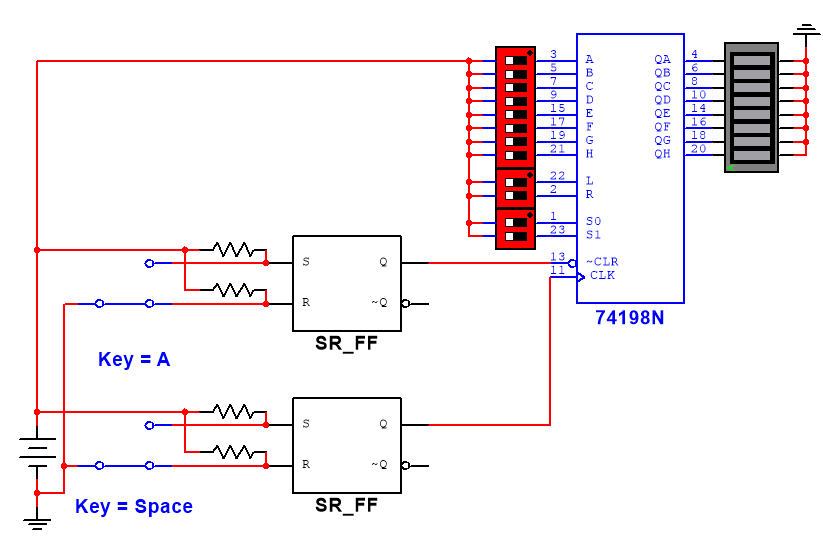
\includegraphics[scale=0.6]{images/image-2.png}
    \captionof{figure}{К155ИР13}
\end{figure}

\subsection*{Тестирование}
\addcontentsline{toc}{subsection}{Тестирование}


\textbf{Режим записи}. Для тестирования режима записи выставим входы $S_1=1,S_0=1$, 
на информационные входы подадим какое либо значение. По положительному перепаду ключа на вход
CLK ожидаем на LED индикации соответвующее значение.  

\begin{figure}[H]
    \centering
    \subcaptionbox{До перепада}{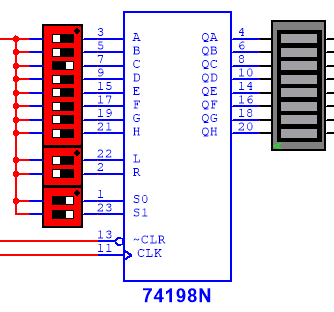
\includegraphics[scale=0.6]{images/image-4.png}}%
    \hspace{40mm}
    \subcaptionbox{После перепада}{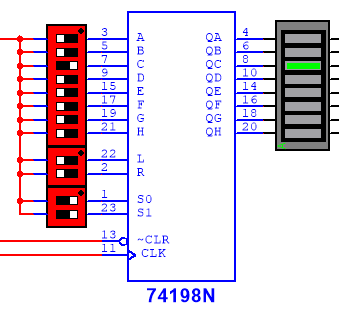
\includegraphics[scale=0.6]{images/image-5.png}}%
    \caption{Режим записи}
\end{figure}
\newpage

\textbf{Сдвиг вправо}. Для режима работы 'сдвиг вправо' выставим входы $S_1=1,S_0=0$. На табло отображено
ранее выставленное значение, после перепада ожидаем сдвиг вправо.

\begin{figure}[H]
    \centering
    \subcaptionbox{До перепада}{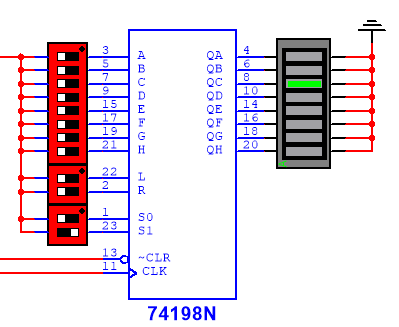
\includegraphics[scale=0.6]{images/image-7.png}}%
    \hspace{40mm}
    \subcaptionbox{После перепада}{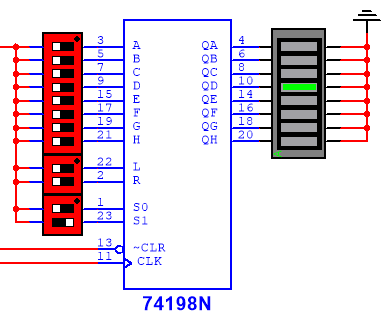
\includegraphics[scale=0.6]{images/image-6.png}}%
    \caption{Сдвиг вправо}
\end{figure}

\textbf{Сдвиг влево}. Для режима работы 'сдвиг влево' выставим входы $S_1=0,S_0=1$. На табло отображено
значение выставленное на прошлом шагу, после перепада ожидаем сдвиг влево.

\begin{figure}[H]
    \centering
    \subcaptionbox{До перепада}{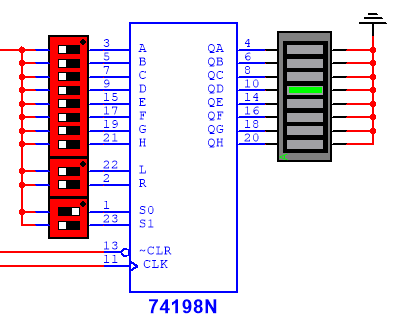
\includegraphics[scale=0.6]{images/image-8.png}}%
    \hspace{40mm}
    \subcaptionbox{После перепада}{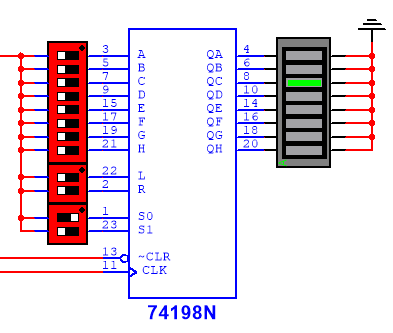
\includegraphics[scale=0.6]{images/image-9.png}}%
    \caption{Сдвиг влево}
\end{figure}

\textbf{Режим храненя}. Для режима работы 'хранение' выставим входы $S_1=0,S_0=0$. На табло отображено
значение выставленное на прошлом шагу, после перепада значение будет сохранятся.

\newpage

\textbf{Порязрядная запись со сдвигом вправо}. Для данного режима работы необходимо выставить режим работы
'сдвиг вправо' ($S_1=1,S_0=0$) и подать сигнал на вход R. На каждом перепаде ожидаем поэтапную запись со сдвигом вправо.

\begin{figure}[H]
    \centering
    \subcaptionbox{До перепада}{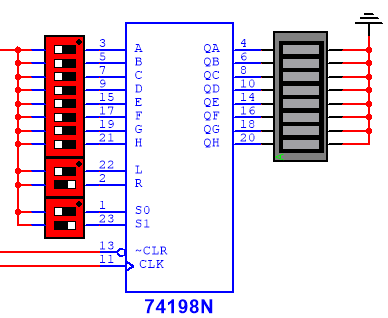
\includegraphics[scale=0.7]{images/image-10.png}}%
    \hspace{20mm}
    \subcaptionbox{Первый перепад}{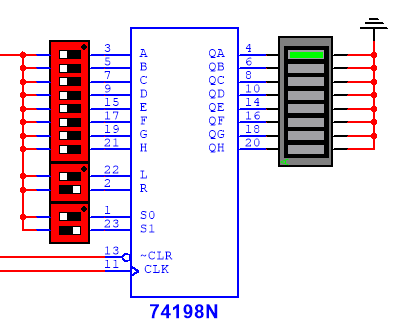
\includegraphics[scale=0.7]{images/image-11.png}}%
    \hspace{20mm}
    \subcaptionbox{Второй перепад}{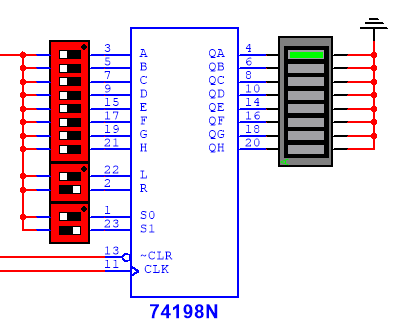
\includegraphics[scale=0.7]{images/image-11.png}}%
    \hspace{20mm}
    \subcaptionbox{Третий перепад}{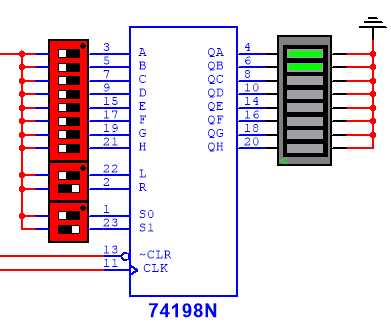
\includegraphics[scale=0.7]{images/image-12.png}}%
    \caption{Порязрядная запись со сдвигом вправо}
\end{figure}

\newpage

\textbf{Порязрядная запись со сдвигом влево}. Для данного режима работы необходимо выставить режим работы
'сдвиг влево' ($S_1=0,S_0=1$) и подать сигнал на вход L. На каждом перепаде ожидаем поэтапную запись со сдвигом влево.

\begin{figure}[H]
    \centering
    \subcaptionbox{До перепада}{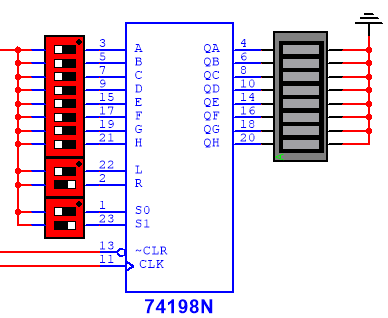
\includegraphics[scale=0.7]{images/image-10.png}}%
    \hspace{20mm}
    \subcaptionbox{Первый перепад}{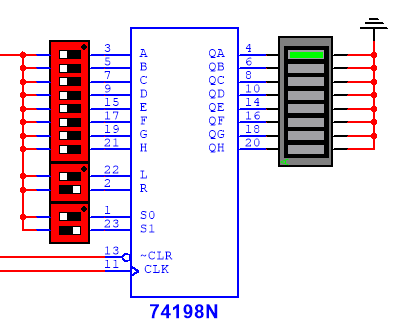
\includegraphics[scale=0.7]{images/image-11.png}}%
    \hspace{20mm}
    \subcaptionbox{Второй перепад}{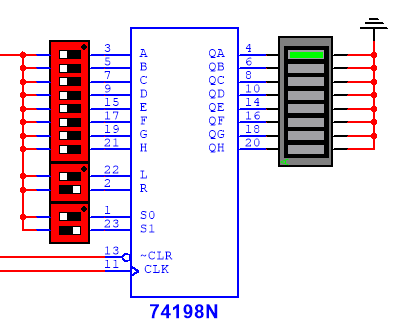
\includegraphics[scale=0.7]{images/image-11.png}}%
    \hspace{20mm}
    \subcaptionbox{Третий перепад}{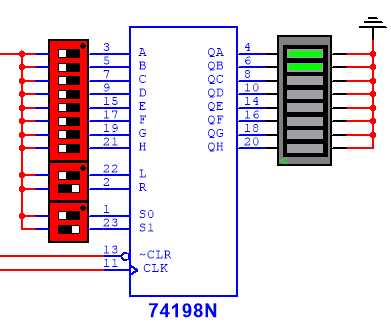
\includegraphics[scale=0.7]{images/image-12.png}}%
    \caption{Порязрядная запись со сдвигом влево}
\end{figure}

\newpage

\subsection*{Коьцевой регистр}
\addcontentsline{toc}{subsection}{Коьцевой регистр}

Далее схема была модифицирована таким образом, чтобы на базе ИС К155ИР13 был
получен универсальный кольцевой регистр. Для этого было учтено, что если
осуществляется сдвиг влево и на выходе A единица, то на выходе H должна будет появиться
единица. Аналогично, если осуществляется сдвиг вправо и на выходе H единица, то на
выходе A должна будет появиться единица. Ключи DL и DR в случае универсального
кольцевого регистра не нужны.

\begin{figure}[h!]
    \centering
    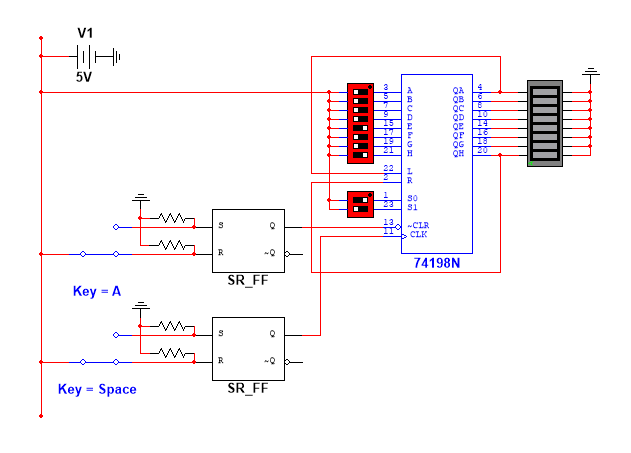
\includegraphics[scale=0.7]{images/image-3.png}
    \captionof{figure}{Универсальный кольцевой регистр}
\end{figure}

\textbf{Кольцевой сдвиг вправо}. Для проверки кольцевого сдвига право выставим пограничное значение 
через режим записи, затем выставим режим работы 'сдвиг вправо'. Ожидаем, что значение индикатора 
изменится с первого разряда на восьмой.

\begin{figure}[H]
    \centering
    \subcaptionbox{До перепада}{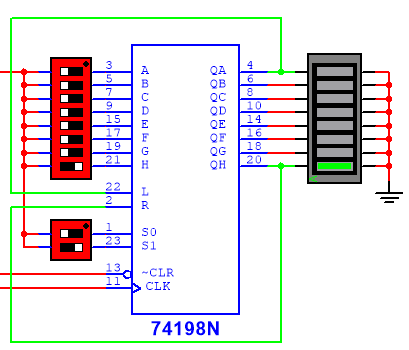
\includegraphics[scale=0.6]{images/image-18.png}}%
    \hspace{30mm}
    \subcaptionbox{После перепада}{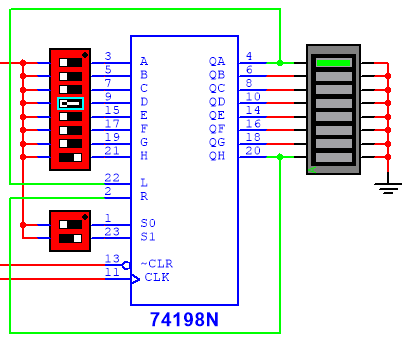
\includegraphics[scale=0.6]{images/image-19.png}}%
    \caption{Кольцевой сдвиг вправо}
\end{figure}

\textbf{Кольцевой сдвиг влево}. Для проверки кольцевого сдвига влево выставим пограничное значение 
через режим записи, затем выставим режим работы 'сдвиг влево'. Ожидаем, что значение индикатора 
изменится с восьмого разряда на первый.

\begin{figure}[H]
    \centering
    \subcaptionbox{До перепада}{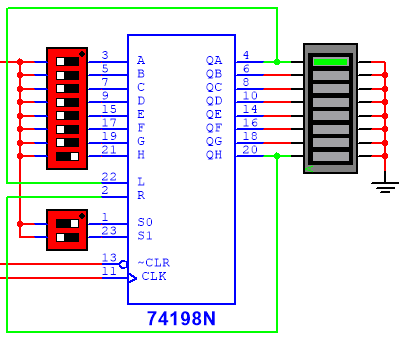
\includegraphics[scale=0.6]{images/image-20.png}}%
    \hspace{30mm}
    \subcaptionbox{После перепада}{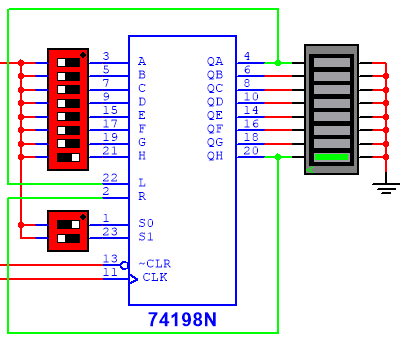
\includegraphics[scale=0.6]{images/image-21.png}}%
    \caption{Кольцевой сдвиг влево}
\end{figure}